%-----------------------------------------------------------------------------------------------------------------------------------------------%
%	The MIT License (MIT)
%
%	Copyright (c) 2015 Jan Küster
%
%	Permission is hereby granted, free of charge, to any person obtaining a copy
%	of this software and associated documentation files (the "Software"), to deal
%	in the Software without restriction, including without limitation the rights
%	to use, copy, modify, merge, publish, distribute, sublicense, and/or sell
%	copies of the Software, and to permit persons to whom the Software is
%	furnished to do so, subject to the following conditions:
%	
%	THE SOFTWARE IS PROVIDED "AS IS", WITHOUT WARRANTY OF ANY KIND, EXPRESS OR
%	IMPLIED, INCLUDING BUT NOT LIMITED TO THE WARRANTIES OF MERCHANTABILITY,
%	FITNESS FOR A PARTICULAR PURPOSE AND NONINFRINGEMENT. IN NO EVENT SHALL THE
%	AUTHORS OR COPYRIGHT HOLDERS BE LIABLE FOR ANY CLAIM, DAMAGES OR OTHER
%	LIABILITY, WHETHER IN AN ACTION OF CONTRACT, TORT OR OTHERWISE, ARISING FROM,
%	OUT OF OR IN CONNECTION WITH THE SOFTWARE OR THE USE OR OTHER DEALINGS IN
%	THE SOFTWARE.
%	
%
%-----------------------------------------------------------------------------------------------------------------------------------------------%


%============================================================================%
%
%	DOCUMENT DEFINITION
%
%============================================================================%

%we use article class because we want to fully customize the page and dont use a cv template
\documentclass[10pt,A4]{article}


%----------------------------------------------------------------------------------------
%	ENCODING
%----------------------------------------------------------------------------------------

%we use utf8 since we want to build from any machine
\usepackage[utf8]{inputenc}

%----------------------------------------------------------------------------------------
%	LOGIC
%----------------------------------------------------------------------------------------

% provides \isempty test
\usepackage{xifthen}

%----------------------------------------------------------------------------------------
%	FONT
%----------------------------------------------------------------------------------------

% some tex-live fonts - choose your own

\usepackage[defaultsans]{droidsans}
% \usepackage[default]{comfortaa}
% \usepackage{cmbright}
% \usepackage[default]{raleway}
% \usepackage{fetamont}
% \usepackage[default]{gillius}
% \usepackage[light,math]{iwona}
% \usepackage[thin]{roboto} 


% set font default
\renewcommand*\familydefault{\sfdefault} 	
\usepackage[T1]{fontenc}

% more font size definitions
\usepackage{moresize}

\usepackage{fontawesome}

%----------------------------------------------------------------------------------------
%	PAGE LAYOUT  DEFINITIONS
%----------------------------------------------------------------------------------------

%debug page outer frames
%\usepackage{showframe}


%define page styles using geometry
\usepackage[a4paper]{geometry}

% for example, change the margins to 2 inches all round
\geometry{top=1cm, bottom=-.6cm, left=0.4cm, right=1cm} 


%less space between header and content
\setlength{\headheight}{-5pt}


%customize entries left, center and right
%\lhead{}
%\chead{ \small{Jan Küster  $\cdot$ Consultant and Software Engineer $\cdot$  Bremen, Germany  $\cdot$  \textcolor{sectcol}{\textbf{info@jankuester.com}}  $\cdot$ +49 176 313 *** **}}
%\rhead{}


%indentation is zero
\setlength{\parindent}{0mm}

%----------------------------------------------------------------------------------------
%	TABLE /ARRAY DEFINITIONS
%---------------------------------------------------------------------------------------- 

%for layouting tables
\usepackage{multicol}
\usepackage{multirow}

%extended aligning of tabular cells
\usepackage{array}

\newcolumntype{x}[1]{%
>{\raggedleft\hspace{0pt}}p{#1}}%


%----------------------------------------------------------------------------------------
%	GRAPHICS DEFINITIONS
%---------------------------------------------------------------------------------------- 

%for header image
\usepackage{graphicx}

%for floating figures
\usepackage{wrapfig}
\usepackage{float}
%\floatstyle{boxed} 
%\restylefloat{figure}

%for drawing graphics
\usepackage{tikz}
\usetikzlibrary{shapes, backgrounds, mindmap, trees}

%----------------------------------------------------------------------------------------
%	Color DEFINITIONS
%---------------------------------------------------------------------------------------- 
\usepackage{transparent}
\usepackage{color}

%accent color
\definecolor{complcol}{RGB}{150,100,20}

% dark background color
% \definecolor{bgcol}{RGB}{110,110,110}
% 
% light background / accent color
% \definecolor{softcol}{RGB}{225,225,225}
% 
% \definecolor{sectcol}{RGB}{0,120,150}

%
%accent color
\definecolor{sectcol}{RGB}{255,150,10}

%dark background color
\definecolor{bgcol}{RGB}{110,110,110}

%light background / accent color
\definecolor{softcol}{RGB}{225,225,225}
%


%Package for links, must be the last package used
\usepackage[]{hyperref}

\hypersetup{
    pdftitle={Nazar Gerasymchuk CV},    % title
    pdfauthor={Nazar Gerasymchuk},     % author
    pdfsubject={CV},   % subject of the document
    pdfcreator={Nazar Gerasymchuk},   % creator of the document
    colorlinks=false,       % false: boxed links; true: colored 
    urlbordercolor=orange,
    pdfborder={0 0 0},
    pdfborderstyle={/S/U/W 1}
}

%============================================================================%
%
%
%	DEFINITIONS
%
%
%============================================================================%

% returns minipage width minus two times \fboxsep
% to keep padding included in width calculations
\newcommand{\mpwidth}{\linewidth-\fboxsep-\fboxsep}
	

%----------------------------------------------------------------------------------------
% 	ARROW GRAPHICS in Tikz
%----------------------------------------------------------------------------------------

% a six pointed arrow poiting to the left
\newcommand{\tzlarrow}{(0,0) -- (0.2,0) -- (0.3,0.2) -- (0.2,0.4) -- (0,0.4) -- (0.1,0.2) -- cycle;}

% include the left arrow into a tikz picture
% param1: fill color
%
\newcommand{\larrow}[1]
{\begin{tikzpicture}[scale=0.58]
    \filldraw[fill=#1!100,draw=#1!100!black]  \tzlarrow
 \end{tikzpicture}
}

% a six pointed arrow poiting to the right
\newcommand{\tzrarrow}{ (0,0.2) -- (0.1,0) -- (0.3,0) -- (0.2,0.2) -- (0.3,0.4) -- (0.1,0.4) -- cycle;}

% include the right arrow into a tikz picture
% param1: fill color
%
\newcommand{\rarrow}
{
\begin{tikzpicture}[scale=0.7]
    \filldraw[fill=sectcol!100,draw=sectcol!100!black] \tzrarrow
 \end{tikzpicture}
}

%----------------------------------------------------------------------------------------
%	custom sections
%----------------------------------------------------------------------------------------

% create a coloured box with arrow and title as cv section headline
% param 1: section title
%
\newcommand{\cvsection}[1]
{
\colorbox{sectcol}{\mystrut \makebox[1\mpwidth][l]{
\larrow{bgcol} \hspace{-8pt} \larrow{bgcol} \hspace{-8pt} \larrow{bgcol} \textbf{\textcolor{white}{\uppercase{#1}}}\hspace{4pt}
}}\\
}

% create a coloured arrow with title as cv meta section section
% param 1: meta section title
%
\newenvironment{metasection}[1] {
	\vspace{6pt}
	\begin{center}
		\textcolor{white}{\large{\textbf{\uppercase{#1}}}}\\
	\normalsize
	\parbox{0.7\mpwidth}{\textcolor{white}	\hrule}
}{\end{center}}

%----------------------------------------------------------------------------------------
%	 CV EVENT
%----------------------------------------------------------------------------------------

% creates a stretched box as cv entry headline followed by two paragraphs about 
% the work you did
% param 1:	event time i.e. 2014 or 2011-2014 etc.
% param 2:	event name (what did you do?)
% param 3:	institution (where did you work / study)
% param 4:	what was your position
% param 5:	some words about your contributions
%
\newcommand{\cvevent}[5]
{
\vspace{8pt}
	\begin{tabular*}{1\mpwidth}{p{0.55\mpwidth}  x{0.42\mpwidth}}
 	\textcolor{black}{\textbf{#2}} & \textcolor{complcol}{\textbf{#3},} \textcolor{bgcol}{#1} 

	\end{tabular*}
\vspace{-12pt}
\textcolor{softcol}{\hrule}
\vspace{6pt}
	\begin{tabular*}{0.5\mpwidth}{p{\mpwidth}}
\larrow{softcol} \textbf{#4}\\[3pt]
\larrow{softcol} #5\\[3pt]
	\end{tabular*}

}

% creates a stretched box as cv entry headline followed by two paragraphs about 
% the work you did
% param 1:	event time i.e. 2014 or 2011-2014 etc.
% param 2:	event name (what did you do?)
% param 3:	institution (where did you work / study)
% param 4:	what was your position
% param 5:	some words about your contributions
%
\newcommand{\cvedu}[4]
{
\vspace{8pt}
	\begin{tabular*}{1\mpwidth}{p{0.55\mpwidth}  x{0.42\mpwidth}}
 	\textcolor{black}{\textbf{#2}} & \textcolor{complcol}{\textbf{#3}} \textcolor{bgcol}{#1} 

	\end{tabular*}
\vspace{-12pt}
\textcolor{softcol}{\hrule}
\vspace{6pt}
	\begin{tabular*}{0.5\mpwidth}{p{\mpwidth}}
\larrow{softcol} #4\\[6pt]
	\end{tabular*}
}

% creates a stretched box as 
\newcommand{\cveventmeta}[2]
{
	\mbox{\mystrut \hspace{87pt}\textit{#1}}\\
	#2
}

%----------------------------------------------------------------------------------------
% CUSTOM STRUT FOR EMPTY BOXES
%----------------------------------------- -----------------------------------------------
\newcommand{\mystrut}{\rule[-.3\baselineskip]{0pt}{\baselineskip}}

%----------------------------------------------------------------------------------------
% CUSTOM LOREM IPSUM
%----------------------------------------------------------------------------------------
\newcommand{\lorem}
{Lorem ipsum dolor sit amet, consectetur adipiscing elit. Donec a diam lectus.}


% use to vertically center content
% credits to: http://tex.stackexchange.com/questions/7219/how-to-vertically-center-two-images-next-to-each-other
\newcommand{\vcenteredinclude}[1]{\begingroup
\setbox0=\hbox{\includegraphics{#1}}%
\parbox{\wd0}{\box0}\endgroup}

% use to vertically center content
% credits to: http://tex.stackexchange.com/questions/7219/how-to-vertically-center-two-images-next-to-each-other
\newcommand*{\vcenteredhbox}[1]{\begingroup
\setbox0=\hbox{#1}\parbox{\wd0}{\box0}\endgroup}

%----------------------------------------------------------------------------------------
%	ICON-SET EMBEDDING
%---------------------------------------------------------------------------------------- 

% at this point we simplify our icon-embedding by simply referring to a set of png images.
% if you find a good way of including svg without conflicting with other packages you can
% replace this part
\newcommand{\icon}[3]{\makebox(#2, #2){\textcolor{#3}{\csname fa#1\endcsname}}}	%icon shortcut
\newcommand{\icontext}[4]{ 						%icon with text shortcut
	\vcenteredhbox{\icon{#1}{#2}{#4}} \vcenteredhbox{\textcolor{#4}{#3}}
}
\newcommand{\iconhref}[5]{ 						%icon with website url
    \vcenteredhbox{\icon{#1}{#2}{#5}} \href{#4}{\textcolor{#5}{#3}}
}

\newcommand{\iconemail}[5]{ 						%icon with email link
    \vcenteredhbox{\icon{#1}{#2}{#5}} \href{mailto:#4}{\textcolor{#5}{#3}}
}



%============================================================================%
%
%
%
%	DOCUMENT CONTENT
%
%
%
%============================================================================%
\begin{document}
\fcolorbox{white}{white}{\begin{minipage}[c][0.95\textheight][t]{0.69\linewidth}


%---------------------------------------------------------------------------------------
%	TITLE HEADLINE
%----------------------------------------------------------------------------------------
\vspace{-3pt}
% use this for multiple words like working titles etc.
%\hspace{-0.25\linewidth}\colorbox{bgcol}{\makebox[1.5\linewidth][c]{\hspace{46pt}\HUGE{\textcolor{white}{\uppercase{M.Sc. Jan Küster}} } \textcolor{sectcol}{\rule[-1mm]{1mm}{0.9cm}} \parbox[b]{5cm}{   \large{ \textcolor{white}{{IT Consultant}}}\\
% \large{ \textcolor{white}{{JS Fullstack Engineer}}}}
%}}

% use this for single words, e.g. CV or RESUME etc.
\colorbox{bgcol}{
    \makebox[\mpwidth-2.1mm][c]{
        \huge{\textcolor{white}{\uppercase{Nazar Gerasymchuk}} 
    } 
    \textcolor{sectcol}{\rule[-1mm]{1mm}{0.8cm}} 
    \LARGE{\textcolor{white}{Programmer} } }
}

%----------------------------------------------------------------------------------------
%	HEADER IMAGE
%----------------------------------------------------------------------------------------


%\hspace{-1.6cm}
%\includegraphics[trim= 0 250 0 270,clip,width=1\linewidth+3.1cm]{myfoto.jpg}	%trimming relative to image size!
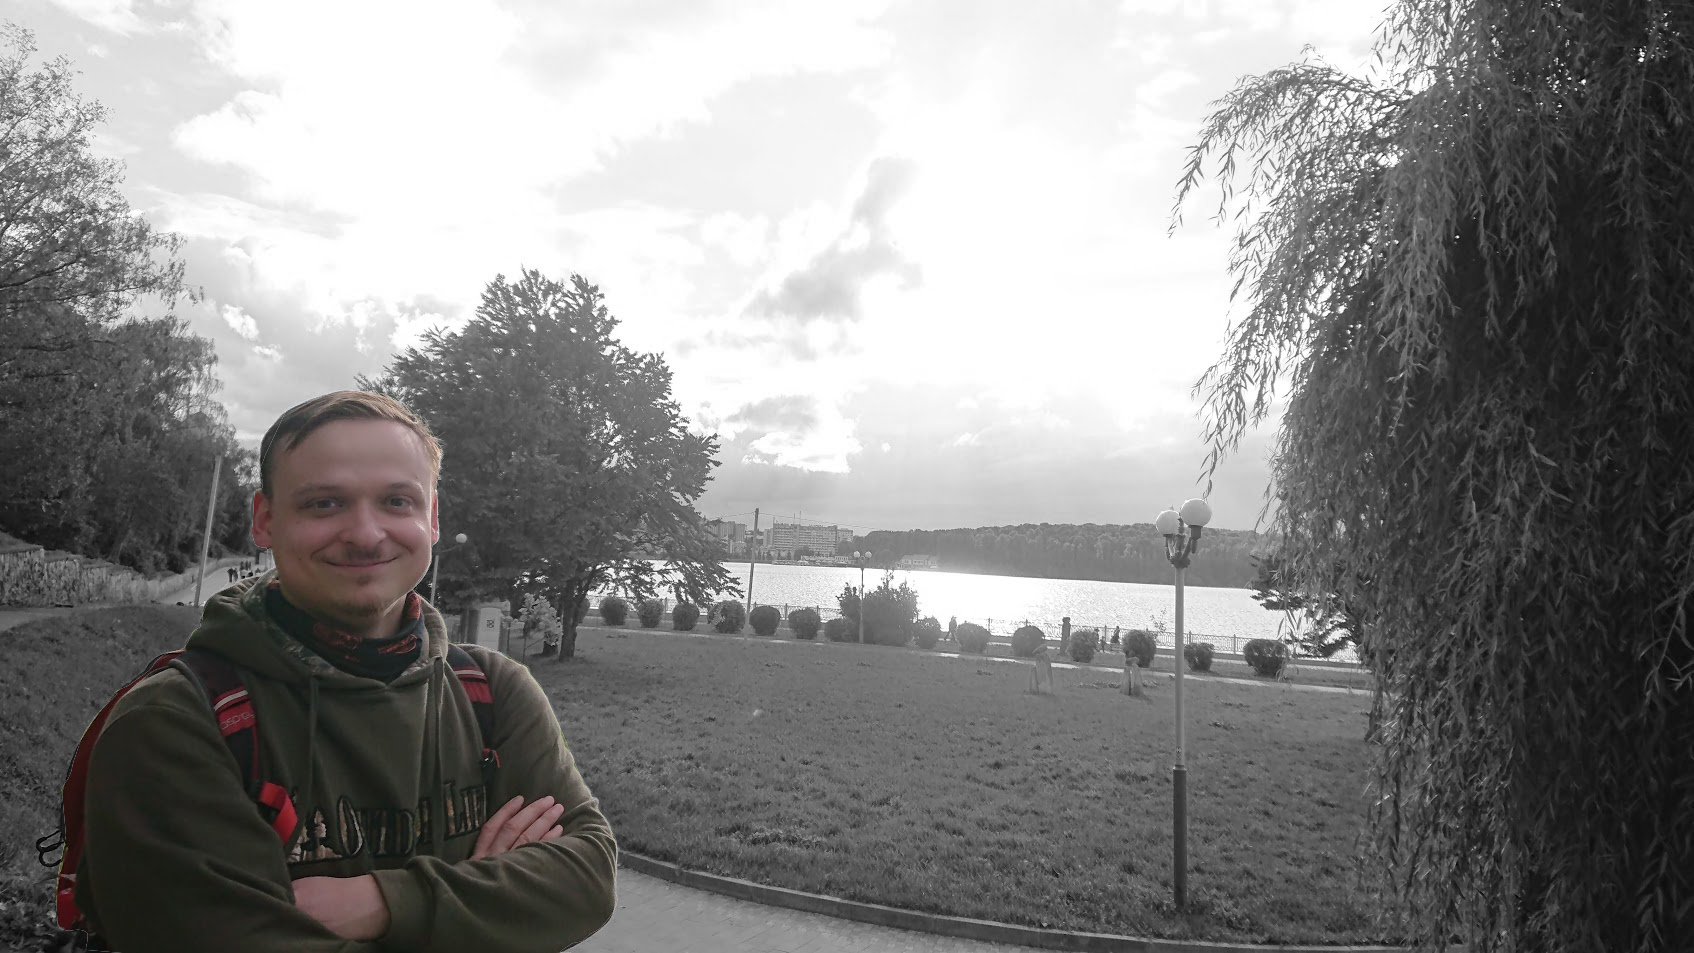
\includegraphics[trim= 0 0 0 250, clip ,width=\linewidth]{ava_test.jpg}	%trimming relative to image size

%---------------------------------------------------------------------------------------
%	SUMMARY
%----------------------------------------------------------------------------------------
\transparent{0.85}%
\vspace{-130pt}
\hspace{0.4\linewidth}
\colorbox{bgcol}{
	\parbox{0.5\linewidth}{
		\transparent{1}%
		\begin{center}
		\larrow{sectcol}\larrow{sectcol}
		\textcolor{white}{
Each time I hugely enjoy when some non-trivial
the real-life task enters my way, and I can solve it by math and/or programming language.
		}
		\end{center}
	}
}
\vspace{60pt}

%============================================================================%
%
%	CV SECTIONS AND EVENTS (MAIN CONTENT)
%
%============================================================================%

%---------------------------------------------------------------------------------------
%	STATUS
%----------------------------------------------------------------------------------------
\cvsection{Moto}

<<\ldots I don't like it when impossible things are explained away by impossible causes. You know, Occam's razor (logical principle of economy of thought). Otherwise you come up with God knows what\ldots>>
\vspace{-4mm}
\begin{flushright}  
<<Definitely Maybe>> A.~\&{}~B.~Strugatsky
\end{flushright}



\vspace{12pt}

%---------------------------------------------------------------------------------------
%	EXPERIENCE
%----------------------------------------------------------------------------------------
\cvsection{Experience}

%
\cvevent{2018--\ldots}{CEO, Enterprener, Developer}{Trola Family}%
{Device creation, R'n'D, Embedded, UI, UX, CI, PM, Documentation.}%
{Research, development of device on Allwinner H3 with SPI LCD, I2C touch and USB host. This work involves: embedded Linux;  custom PCB preparation; Armbian build \& customization; custom cross-toolchain for Qt~5.12.
}

%\textcolor{softcol}{\hrule}

\cvevent{2014--2018}{C++/Qt/QML developer}{Milo Solutions}%
{Development, R'n'D, PM, Estimations, Client communication, UI, UX, Embedded, Crossplatform, CI/CD, Refactoring, Code review, Documentation}%
{Lots of interesting tasks and projects, PM'ed several of them. Work with different Qt versions (4.6--5.9) on variety of platforms: Windows, Linux, MacOS, Android, iOS, Embed Linux. Done lot of porting (from older Qt to newer, between different platforms etc). Usage of Python and/or Bash for automatisation.}

%\textcolor{softcol}{\hrule}

%
\cvevent{2013}{C++/Qt developer}{<<Google Summer of Code>>}%
{Internship at Mixxx development. Worked on task for rewriting \emph{non-blocking database access}.}%
{Qt 4.8 on Linux/Windows. Usage of $\lambda$ from C++11. Multithreading, scons, git, SQLite, \ldots  }

%\textcolor{softcol}{\hrule}

\cvevent{2008--2011}{Informatics and Robotics group leader}{VO~MAN}%
{Teaching computer science. Organisation. Guidelines preparation.}%
{Informatics and Robotics group leader, teaching practice: computer science, algorithmization, programming (Pascal), robotics (based on LEGO NXT).}

\vspace{12pt}
%---------------------------------------------------------------------------------------
%	EDUCATION SECTION
%--------------------------------------------------------------------------------------
\cvsection{Education}

\cvedu{2011--2013}{Master of Informatics}{}%
{Taras Shevchenko National University of Kyiv, Department of Cybernetics.}

%\textcolor{softcol}{\hrule}

%
\cvedu{2007--2011}{Bacholer of Informatics}{}%
{Lesya Ukrainka Volyn National University, Department of Mathematics.}

%\textcolor{softcol}{\hrule}


\end{minipage}}%
\fcolorbox{white}{sectcol}{\begin{minipage}[c][0.95\textheight][t]{0.33\linewidth}


\begin{metasection}{Contact}

	\iconhref{LocationArrow}{12}{Lutsk/Ternopil, Ukraine}{https://goo.gl/maps/wcAE21i7WHU2}{white}\\[4pt]
	\iconhref{LinkedinSquare}{12}{gerasymchuknazar}{https://www.linkedin.com/in/gerasymchuknazar}{white}\\[4pt]
	\iconemail{Envelope}{12}{troyan3@gmail.com}{troyan3@gmail.com}{white}\\[4pt]
	\iconhref{MousePointer}{12}{http://trola.org/blog}{www.trola.org}{white}\\[4pt]
	\iconhref{Github}{12}{troyane}{https://github.com/troyane}{white}\\[4pt]
	\iconhref{Gitlab}{12}{tr0}{https://gitlab.com/tr0}{white}\\[4pt]
\end{metasection}
	
%----------------------------------------------------------------------------------------
%	META SECTION
%----------------------------------------------------------------------------------------

\begin{metasection}{Languages}

    \textcolor{white}{
        \textbf{English} -- upper intermediate \\[4pt]
        \textbf{Ukrainian} -- native \\[4pt]
        \textbf{Russian} -- advanced \\[4pt]
    }
\end{metasection}


\begin{metasection}{Technologies}

\textcolor{white}{
\icontext{Code}{12}{C++, Qt, QtQuick/QML, Python}{white} 
\\[4pt]
\icontext{Gear}{12}{SQL, CSS, XML, JSON, Flask, Bash}{white} 
\\[4pt]
\icontext{Gears}{12}{Regex, JavaScript}{white} 
\icontext{CodeFork}{12}{Git}{white} 
\icontext{Linux}{12}{Linux}{white} 
\\[4pt]
\icontext{Plug}{12}{RPi, NanoPi, Arduino, WiringPi}{white}
\\[4pt]
\icontext{Code}{12}{OOP, UML}{white} 
}
\end{metasection}

\begin{metasection}{Tools}

\textcolor{white}{
\icontext{Code}{12}{QtCreator}{white}
\\[4pt]
\icontext{Columns}{12}{Redmine, Jira, Kanban}{white}\\[4pt]
\icontext{Sitemap}{12}{Apache, Flask, SSH, Hugo}{white}\\[4pt]
\icontext{PaintBrush}{12}{Inkscape, GIMP}{white}\\[4pt]
\LaTeX
}
\end{metasection}

\begin{metasection}{Soft skills}

\textcolor{white}{
    Teamwork, positive attitude, self-confidence, flexibility, mindfulness, creativity
}
\end{metasection}


\begin{metasection}{Interests}

\iconhref{StackOverflow}{12}{StackOverflow admirer, $\sim$5K}{https://stackoverflow.com/users/867349/troyane}{white} \\[4pt]
\icontext{MousePointer}{12}{OpenSource enthusiast \small{from 2007}}{white}\\[4pt]
\icontext{Tasks}{12}{Exercism student}{white}\\[4pt]
\icontext{Linux}{12}{Linuxoid}{white}\\[4pt]

\icontext{Book}{12}{Reading}{white}
\icontext{Cube}{12}{Board games}{white}\\[4pt]

\icontext{Suitcase}{12}{Travelling, hiking}{white}
\icontext{Bicycle}{12}{Cycling}{white}\\[4pt]

\icontext{Gamepad}{12}{Gaming, handled}{white}
\icontext{PaintBrush}{12}{Caligraphy}{white}\\[4pt]
\icontext{Headphones}{12}{Sound producer, experimentator}{white}
\end{metasection}

%---------------------------------------------------------------------------------------
%	QR CODE (optional)
%----------------------------------------------------------------------------------------

\vspace{0pt}
\begin{center}

\includegraphics[width=0.35\mpwidth]{qrcode}
\end{center}

\end{minipage}}

%-------------------------------------------------------------------------------------------------
%	ARTIFICIAL FOOTER (fancy footer cannot exceed linewidth) 
%--------------------------------------------------------------------------------------------------

\null
\vspace*{\fill}
\hspace{-0.25\linewidth}\colorbox{bgcol}{\makebox[1.5\linewidth][c]{\mystrut \small \textcolor{white}{You can find this CV (code \& pdf) at \iconhref{Github}{12}{my repo.}{https://github.com/troyane/CV}{white} }}}

%============================================================================%
%
%
%
%	DOCUMENT END
%
%
%
%============================================================================%
\end{document}
